\subsection{FinalDocument}

Se corresponde con todos los datos almacenados acerca de una ley. Es un objeto complejo constituído por otros más pequeños.

\begin{figure}[H]
\centerline{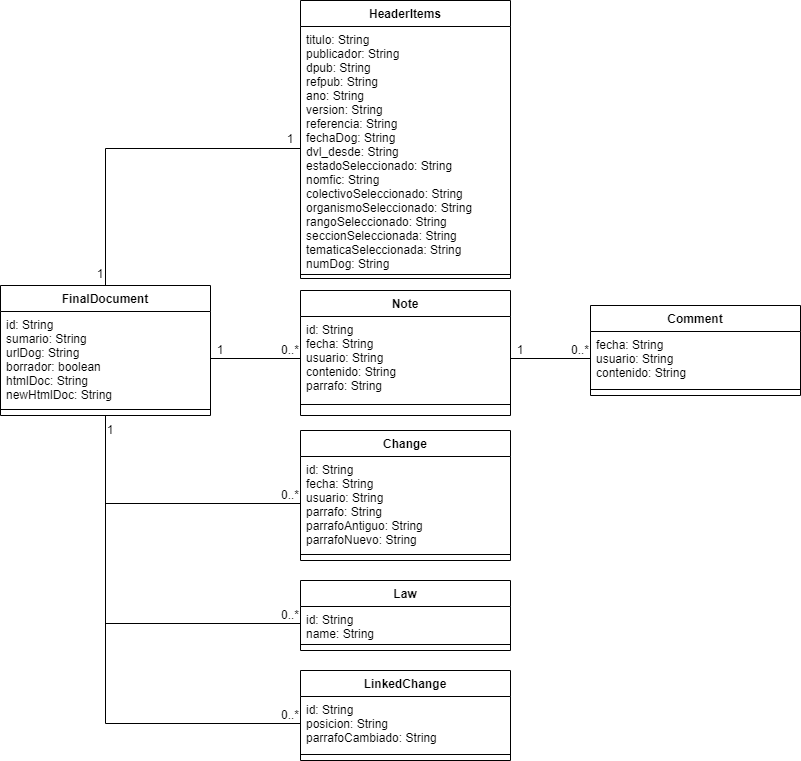
\includegraphics[width=15cm]{figuras/diseño/FinalDocument.png}}
\caption{Documento FinalDocument.}
\label{enlaceFinalDocument}
\end{figure}

La \hyperref[enlaceFinalDocument]{Figura 3.6} representa como se constituye el documento {\it FinalDocument} de la aplicación.
\\

Una ley está formada por un id, sumario, enlace de la ley en el DOG, indicador de si la ley es un borrador, documento HTML, y el documento HTML modificado. 
\\

A su vez, esta contiene un conjunto de datos de cabecera (HeaderItems), que son metadatos que conforman la ley. Entre ellos encontramos, por ejemplo, el título, publicador, fecha de publicación en el DOG, etc.
\\

Las leyes están formadas o no por una lista de notas (Note). Sus atributos son el id, fecha, usuario, contenido, y el párrafo sobre el que se realizan. Estas a su vez pueden contener una lista de comentarios (Comment), que contienen la fecha, usuario y contenido del propio comentario.
\\

También pueden tener o no cambios (Change), donde se indica su id, fecha, usuario, párrafo al que afectan, párrafo antiguo y el párrafo nuevo.
\\

Con respecto a las leyes vinculadas (Law), se almacena su id y el nombre. Sobre estas se pueden realizar cambios (LinkedChange), donde se almacena el id, párrafo al que afectan, y el contenido del nuevo párrafo.